\newpage

\section*{ $^{98}$Mo(n,$\gamma$)$^{99}$Mo }

Power Level: 100 kW(th) \\
Time at Power: 60.0 m \\
Wait Time: 24.0 h \\
Counting Time: 10.0 m \\
Total Activity at Removal: 4.80e+00 $\mu Ci$

\begin{table*}[h]
\centering
\begin{tabular}{ |c|c|c|c|c|c| }
 \hline
 Position & Mass $mg$ & Counting Activity $\mu Ci$ & Area (Counts) & Error \% \\
 \hline 
 1 & 2.95 & 8.46e-01 & 6.86e+04 & 0.3817 \\ 
\hline
 2 & 2.95 & 1.22e+00 & 9.91e+04 & 0.3176 \\ 
\hline
 3 & 2.95 & 1.14e+00 & 9.26e+04 & 0.3286 \\ 
\hline
 4 & 2.95 & 5.51e-01 & 4.47e+04 & 0.4731 \\ 
\hline
\end{tabular}
\end{table*}

\begin{figure}[h]
\centering
\begin{subfigure}{.5\textwidth}
  \centering
     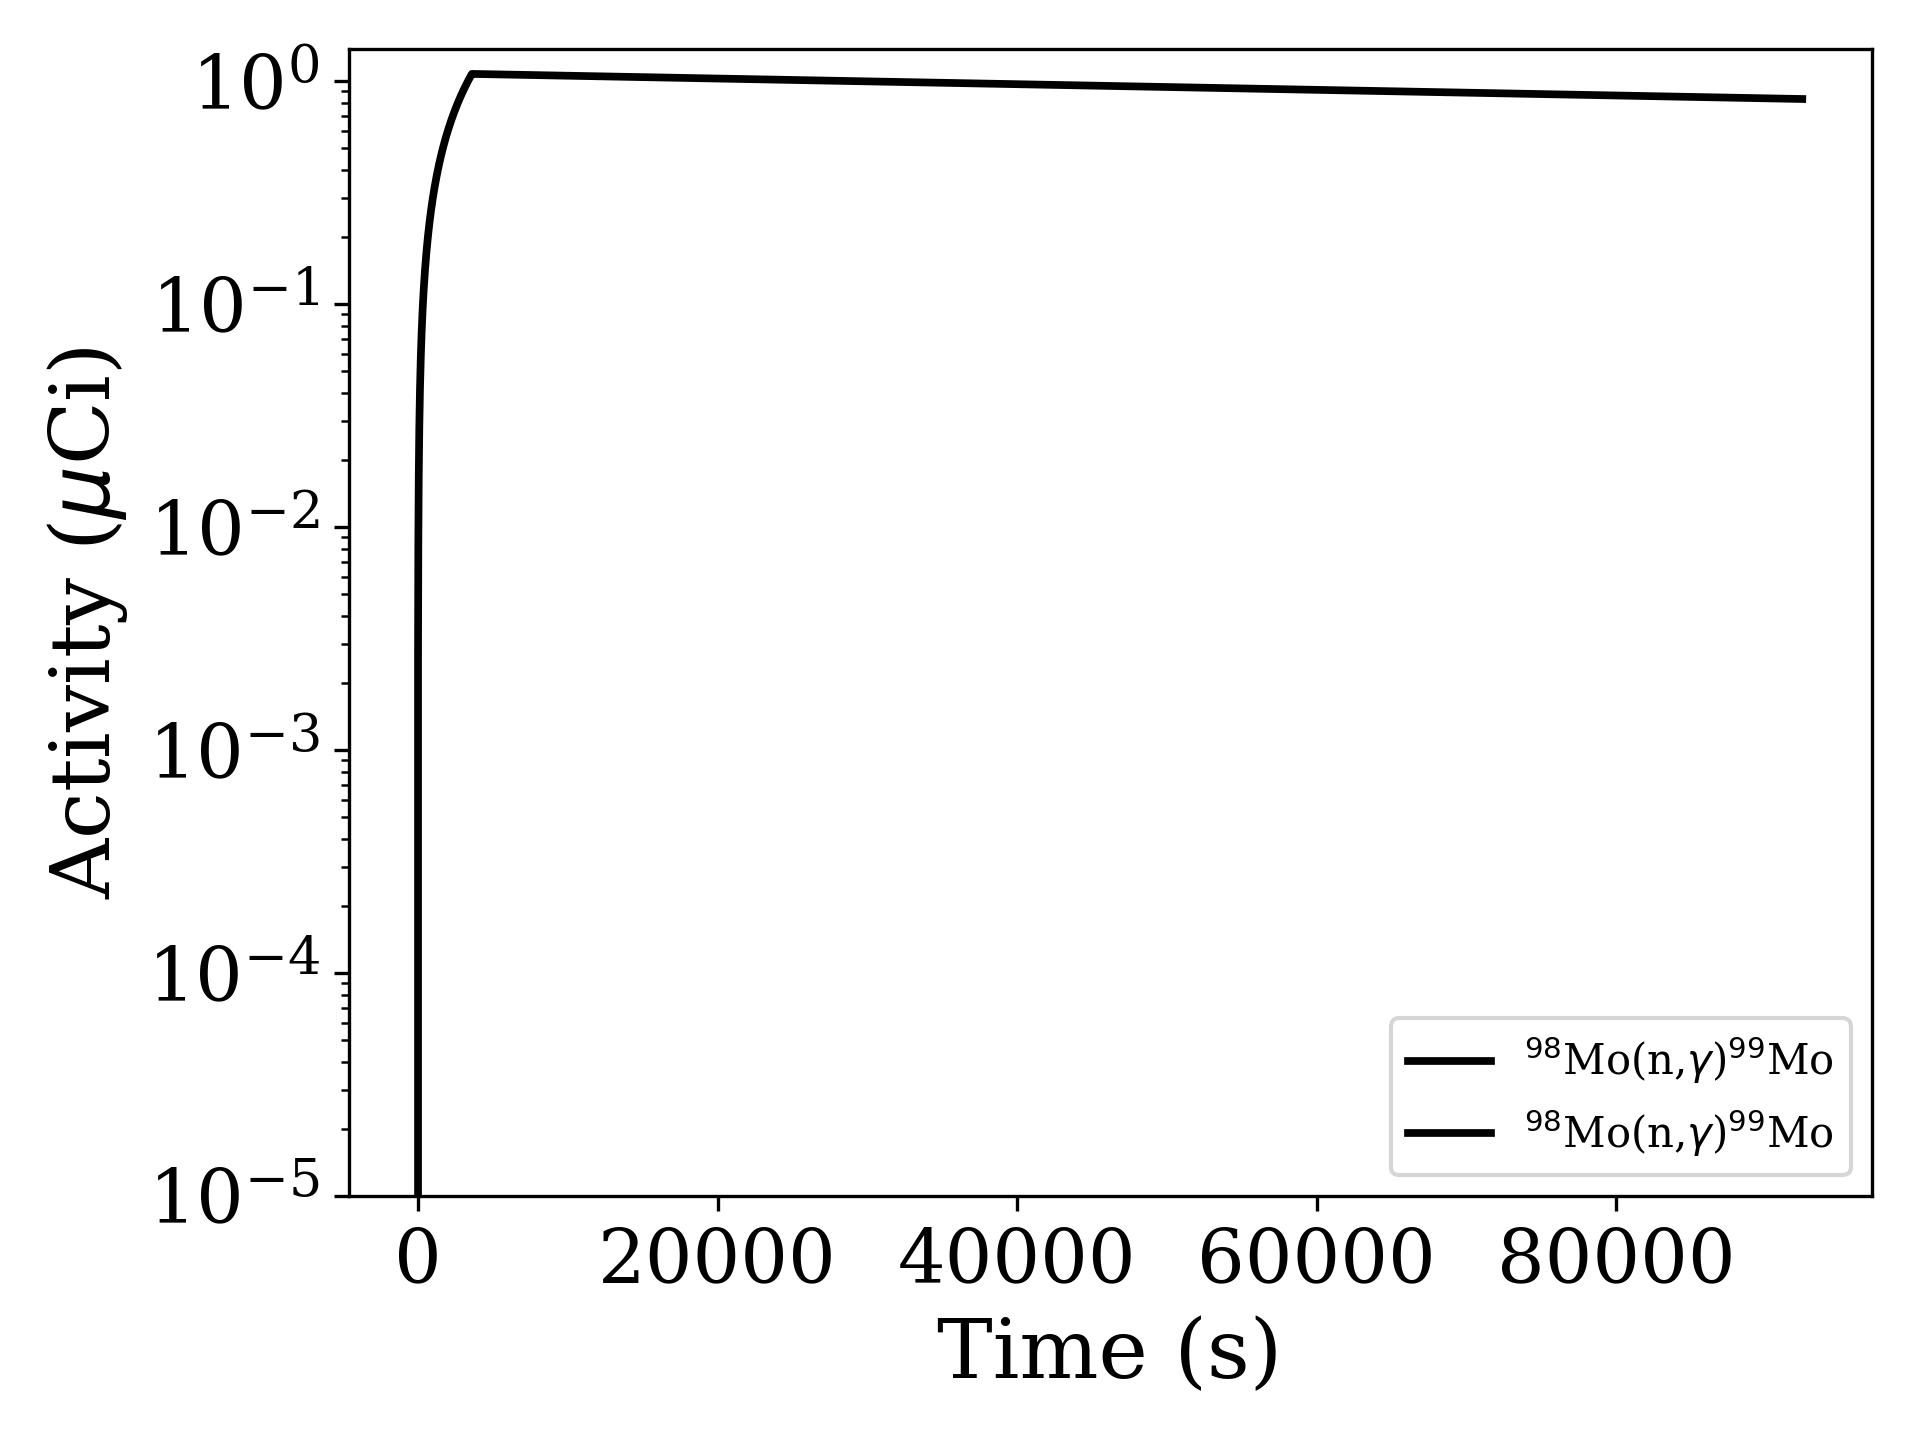
\includegraphics[width=.8\textwidth]{plot/Mo-98(n,gamma)Mo-99_wisconsin1} 

  \caption{Activity}
\end{subfigure}%
\begin{subfigure}{.5\textwidth}
  \centering
     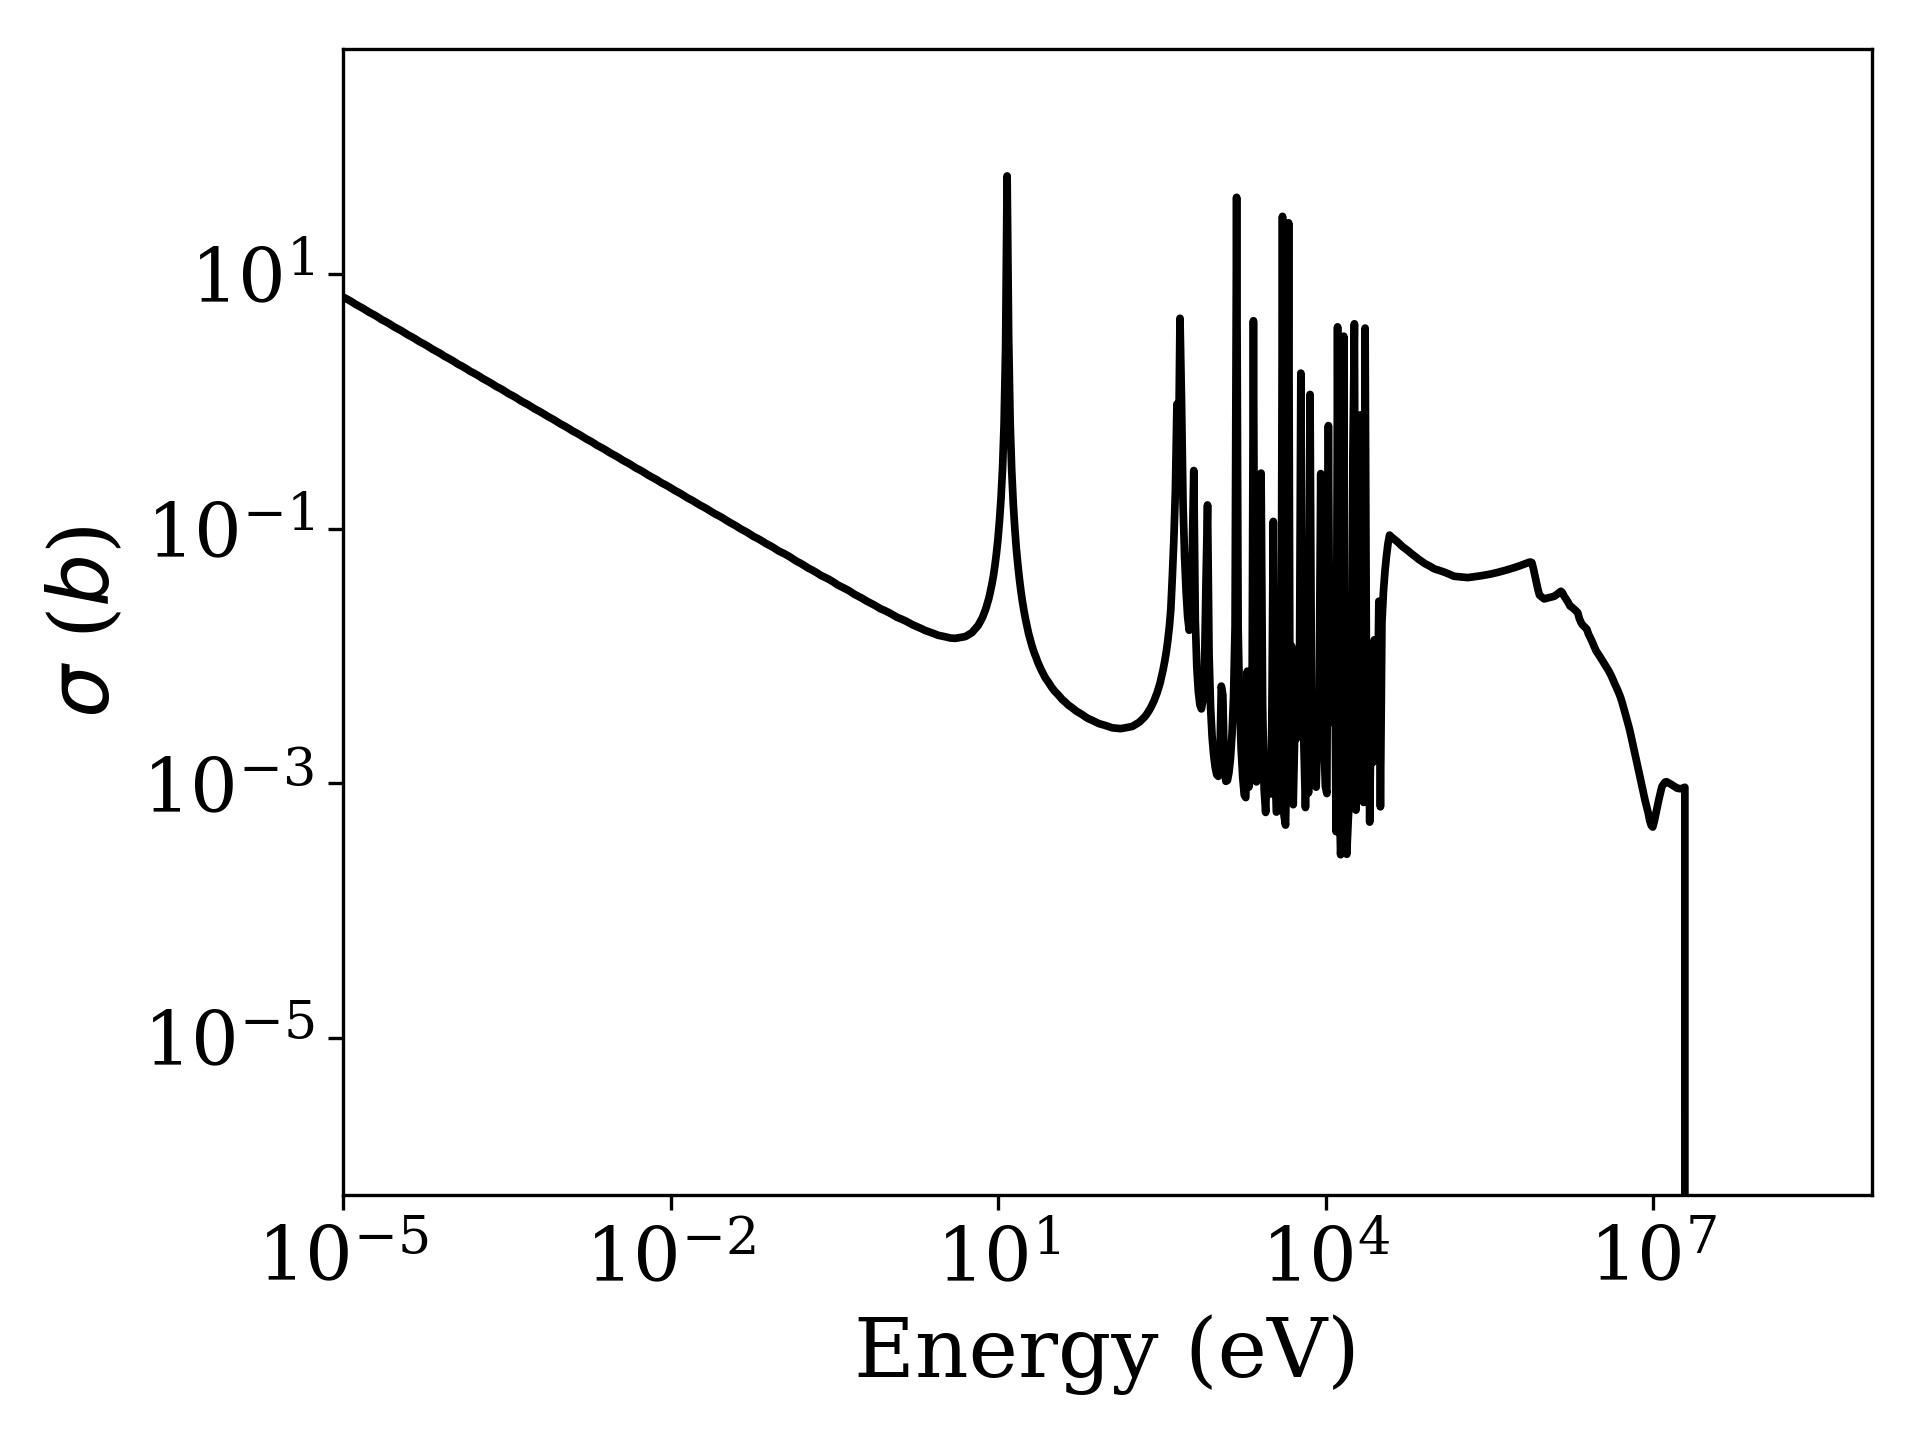
\includegraphics[width=.8\textwidth]{plot/Mo-98(n,gamma)Mo-99} 

  \caption{Cross Section}
\end{subfigure}
\end{figure}

\begin{table*}[h]
\centering
\begin{tabular}{ |c|c|c|c|c|c|c| }
 \hline
 Reaction & T$_{1/2}$ & ROI (eV) & Important Gammas (keV) \\
 \hline 
 $^{98}$Mo(n,$\gamma$)$^{99}$Mo &  2.8 d & 2.96e-02, 2.26e+05 & 740(0.12) \\ 
\hline
\end{tabular}
\end{table*}
